\documentclass[11pt]{article}
\usepackage{mathunal-base}
\mathunalfuente{serif}
\newlist{opciones}{enumerate}{1}
\setlist[opciones]{label=(\alph*),itemsep=1pt,topsep=2pt,leftmargin=1.8em,font=\normalfont}
\newlist{romanos}{enumerate}{1}
\setlist[romanos]{label=\roman*.,itemsep=1pt,topsep=2pt,leftmargin=1.8em,font=\normalfont}

\renewcommand{\examtitulo}{Ecuaciones Diferenciales (1000007) --- Primer examen parcial}
\renewcommand{\examfecha}{Semestre 01-2015, 07 de Marzo de 2015}

\begin{document}

\examheader

\vspace{4pt}
\noindent\textit{Duración: 1 hora y 40 minutos. Instrucciones: No está permitido el uso de calculadora ni de cualquier otro tipo de aparato electrónico, incluyendo teléfonos móviles, los cuales deben permanecer apagados durante el tiempo de duración del examen. Tampoco está permitido hacer preguntas a las personas encargadas de la vigilancia.}

\vspace{6pt}
\noindent\textbf{1. (25\%)} Resuelva el siguiente problema de valor inicial
\[
x^2\frac{dy}{dx}+y^2=xy, \qquad x>0, \qquad y(e)=1.
\]

\vspace{6cm}

\newpage

\noindent\textbf{2. (20\%)} Considere la ecuación diferencial autónoma
\[
\frac{dy}{dt}=y(y-2)(y-4)\equiv f(y), \qquad t\geq 0, \qquad y(0)=y_0,\ 0\leq y_0<\infty.
\]

\begin{opciones}
\item \textbf{(6\%)} Trace la gráfica de $f(y)$ contra $y$.
\item \textbf{(6\%)} Determine los puntos críticos (o soluciones de equilibrio) y clasifíquelos.
\item \textbf{(8\%)} Trace una curva integral en cada una de las regiones del plano $ty$ determinada por las soluciones de equilibrio.
\end{opciones}

\begin{center}
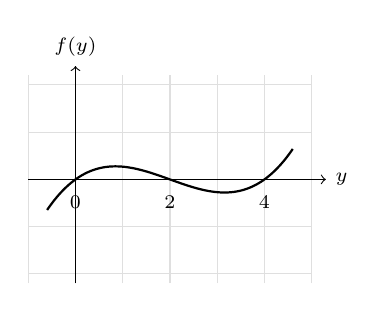
\begin{tikzpicture}[scale=0.6]
\draw[gray!25,thin] (-1,-2.2) grid (5,2.2);
\draw[->] (-1,0) -- (5.3,0) node[right,font=\scriptsize]{$y$};
\draw[->] (0,-2.2) -- (0,2.4) node[above,font=\scriptsize]{$f(y)$};
\draw[thick,domain=-0.6:4.6,samples=80] plot(\x,{0.09*\x*(\x-2)*(\x-4)});
\foreach \x in {0,2,4}{\node[below,font=\scriptsize] at (\x,-0.15){\x};}
\end{tikzpicture}
\hspace{1cm}
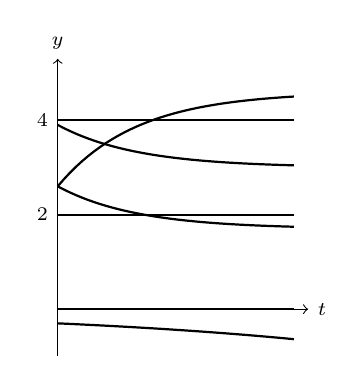
\begin{tikzpicture}[scale=0.6]
\draw[->] (0,0) -- (5.3,0) node[right,font=\scriptsize]{$t$};
\draw[->] (0,-1) -- (0,5.3) node[above,font=\scriptsize]{$y$};
\draw[thick] (0,2) -- (5,2); \node[left,font=\scriptsize] at (0,2){2};
\draw[thick] (0,4) -- (5,4); \node[left,font=\scriptsize] at (0,4){4};
\draw[thick] (0,0) -- (5,0);
\draw[thick,domain=0:5,samples=40] plot(\x,{4.6-2*exp(-0.6*\x)});
\draw[thick,domain=0:5,samples=40] plot(\x,{1.7+0.9*exp(-0.6*\x)});
\draw[thick,domain=0:5,samples=40] plot(\x,{3+0.9*exp(-0.6*\x)});
\draw[thick,domain=0:5,samples=40] plot(\x,{-0.3*exp(0.15*\x)});
\end{tikzpicture}
\end{center}
\nota{Figuras esquemáticas (redibujadas): a la izquierda $f(y)$ contra $y$ (parábola cúbica con raíces en $y=0,2,4$); a la derecha una curva integral representativa en cada una de las 4 regiones que determinan $y=0$, $y=2$, $y=4$ en el plano $ty$.}

\newpage

\noindent\textbf{3. a.} \textbf{(10\%)} Considere la ecuación diferencial
\[
\frac{dy}{dx}=x\sqrt{1-y^2}.
\]
Para cada una de las siguientes condiciones explique, sin resolver la ecuación diferencial, si el teorema de existencia y unicidad garantiza o no la existencia de solución única del problema de valor inicial correspondiente.
\begin{romanos}
\item $y(0)=0$.
\item $y(0)=1$.
\end{romanos}

\vspace{3cm}

\noindent\textbf{b. (20\%)} Resuelva la ecuación diferencial
\[
\frac{dy}{dx}=\frac{y+\sqrt{x^2-y^2}}{x}.
\]

\vspace{6cm}

\newpage

\noindent\textbf{4. (25\%)} Un tanque con capacidad de 200 galones contiene inicialmente 50 galones de agua con 10 libras de sal. Al tanque entra agua con una concentración de sal de $\dfrac{1}{t+50}$ libras de sal por galón a razón de 4 galones por minuto y la mezcla resultante sale del tanque a razón de 3 galones por minuto.

\begin{opciones}
\item \textbf{(7\%)} Halle el volumen de la mezcla en el instante $t$, antes de que la mezcla se derrame.
\item \textbf{(18\%)} Encuentre la cantidad de sal presente en el tanque en el momento que la mezcla comienza a derramarse.
\end{opciones}

\vspace{6cm}

\vfill
\rule{\linewidth}{0.4pt}\\[1pt]
{\scriptsize\textit{Transcripción digital --- MathUNAL}\hfill\textcolor{unalblue}{\textbf{1}}}

\end{document}
